%%% generic article type (pdf)latex file
%%% use together with Makefile

\documentclass[letterpaper]{scrartcl}
\usepackage{natbib}
\usepackage{graphicx}
\usepackage{subcaption}
\usepackage{amsmath,amsfonts,amsthm}
\usepackage{eufrak}
\usepackage{mathabx}
\usepackage{siunitx}
\usepackage{url}
\usepackage{framed}
\usepackage[usenames,dvipsnames,svgnames,table]{xcolor}
\usepackage[colorlinks]{hyperref}
\hypersetup{
     colorlinks   = true,
     urlcolor     = blue,
     linkcolor    = red,
     citecolor    = black
}
\usepackage{enumitem}
\usepackage{booktabs}
\usepackage{cprotect}
\usepackage{minted}

%\usepackage{wrapfig}
%\usepackage{subfig}
\usepackage[format=plain,labelsep=period,font=small,labelfont=bf]{caption}

%------------------------------------------------------------
% assignment
%
\newcommand{\anumber}{2}
%
%------------------------------------------------------------

% hyperref https://en.wikibooks.org/wiki/LaTeX/Hyperlinks#.5Chref
\urlstyle{same}

%% not working yet...
\newcounter{TotalPoints}
\newcounter{TotalBonus}

\newcommand{\BONUS}{\textsc{Bonus: }}
\newcommand{\bonus}[1]{\textbf{[bonus +#1*]}\stepcounter{TotalBonus}}
\newcommand{\points}[1]{\textbf{[#1 points]}\stepcounter{TotalPoints}}
\newenvironment{enuma}{\begin{enumerate}[label=(\alph*)]}{\end{enumerate}}
\newenvironment{enumi}{\begin{enumerate}[label=(\roman*)]}{\end{enumerate}}
\newenvironment{solution}{\par\noindent\P{} }{\ \qedsymbol}

\renewcommand{\vec}[1]{\ensuremath{\mathbf{#1}}}
\newcommand{\pd}[3][]{\left(\frac{\partial #2}{\partial #3}\right)_{#1}}

\DeclareSIUnit{\revolutions}{rev}

\newcommand{\anum}{0\anumber}

\title{{\Large Project \anumber: Soccer Physics for the WIN!}}

\author{{\sffamily\large Project \emph{Comp. Methods Physics} ASU
    PHY494 (2018)}%
  \thanks{Current version of this document: \today. See
    Appendix~\protect\ref{sec:history} for a list of changes since v1
    from March 26, 2018.}}

\date{{\sffamily\large March 26, 2018 -- April 9, 2018}}


\begin{document}
\maketitle

\paragraph{Abstract}

In \emph{soccer} (or \emph{football} for the world outside the US) a
goal is scored when the entire ball fully crosses the goal line
between the goal posts and under the goal cross bar. There are a
number of set-piece situations that can directly lead to goals. Here
we look at two such opportunities that start from a ball at rest: the
\textbf{direct free kick} and the \textbf{corner kick}. You will write
Python code to simulate a realistic flight trajectory of the ball
(including spin and air resistance) and solve the problem to choose
initial kick parameters that could lead to directly scoring a
goal. You will write a \emph{short report} to communicate, discuss and
summarize your reasoning and your results. The work is carried out in
teams of two or three students.

\begin{framed}
  \noindent
  Due Monday, April 9, 2018, 11:59pm.
  \begin{itemize}
  \item Students work in teams of two or three students.
  \item \textbf{Admissible Collaboration:} Students are allowed to
    talk to other students in the class about the project and exchange
    ideas and tips. However, sharing/copying reports or full code
    solutions is not allowed. \textbf{Help from other students must be
      acknowledged in an Acknowledgments section}.  Direct help from
    outside the class is not allowed (except instructor/TA), e.g., you
    cannot ask for solutions (online or in person) but you can use
    books and resources on the internet to solve
    problems. \textbf{Cite all sources}. Code from the class can be
    used without explicit citation or acknowledgement.
  \item Each team should commit their  report (see
    Section~\ref{sec:report}) in \textbf{PDF} format to the team's
    \textbf{GitHub repository}; alternatively, combining report and
    code in a Jupyter notebook is also possible as long as the
    notebook can be read like a report (i.e., not just bullet points
    or short comments). If possible, also generate a PDF from your
    notebook and commit it together with everything else.
  \item The report \emph{must} contain a section
    \textbf{Contributions} at the end where the contributions of all
    team members are summarized. 
  \item Each team should commit and push \textbf{all code} (see
    Section \ref{sec:code}) that is required to reproduce the results
    in the report to their \textbf{GitHub repository}. Include a
    text file \textbf{\texttt{README.txt}} that describes the commands
    to run calculations. The code must run in the standard
    anaconda-based environment used for the class. If it is a Jupyter
    notebook then it should be possible to \emph{Kernel $\rightarrow$
      Restart \& Run All} and to produce all the required figures and
    output.
  \end{itemize}
  Grading will take the following into consideration:
  \begin{itemize}
  \item The code runs and produces correct output.
  \item The report clearly and succinctly describes the question,
    approach, and results and contains sufficient evidence that the
    requirements (see below) have been met.
  \item All team members contributed to the work: assessed by (1)
    Contributions section in the report, (2) commit history of the
    repository and comments in code, (3) short oral examination of
    team members (at instructor's discretion if deemed necessary).
  \item Code from outside sources (see Admissible Collaboration) and
    help is thoroughly attributed (Acknowledgements and References).
  \item \BONUS Additional work that you want to include in an appendix to
    the report or additional simulations for the main report will be
    treated as bonus material and can be awarded bonus points.
  \item \BONUS Elegant and fast code can be awarded bonus points.
  \end{itemize}
\end{framed}

\newpage
\tableofcontents{}

\section{Submission instructions}

\noindent
%  \url{}
\fbox{\parbox{\linewidth}{Submission is to your private \textbf{team
      GitHub repository}. Follow the link provided to you by the
    instructor in order for the repository to be set up: It will have
    the name
    \emph{ASU-CompMethodsPhysics-PHY494/project-2-2018-\emph{YourTeamName}}
    and will only be visible your team and the instructor/TA. Follow the
    instructions below to submit this project.}}
Read the following instructions carefully. Ask if anything is unclear.
\begin{enumerate}
\item \texttt{git clone} your project repository (change
  \emph{YourTeamName} to your team's name)
  \begin{minted}[autogobble]{bash}
    repo="project-2-2018-YourTeamName.git" 
    git clone https://github.com/ASU-CompMethodsPhysics-PHY494/${repo}
  \end{minted}
  %$
  or, if you already have done so, \mintinline{bash}{git pull} from
  within your assignments directory.
\item  Create three sub-directories \texttt{Submission},
  \texttt{Grade}, and
  \texttt{Work}.
\item You can try out code in the \texttt{Work}
  directory but you don't have to use it if you don't want to. Your
  grade with comments will appear in
  \texttt{Grade}.
\item Create your solution in
  \texttt{Submission}. Use Git to \texttt{git
    add} files and \texttt{git commit} changes.

  You can create a PDF file or Jupyter notebook inside the
  \texttt{Submission} directory as well as Python
  code (if required). \textbf{Name your files \texttt{project\anum.pdf} or
    or \texttt{project\anum.ipynb}}, depending on how
  you format your work. Files with code (if requested) should be named
  exactly as required in the assignment.
\item When you are ready to submit your solution, do a final
  \texttt{git status} to check that you haven't forgotten anything,
  commit any uncommitted changes, and \texttt{git push} to your GitHub
  repository. Check on \emph{your} GitHub repository web
  page\footnote{\texttt{https://github.com/ASU-CompMethodsPhysics-PHY494/project-2-2018-\emph{YourTeamName}}}
  that your files were properly submitted.

  You can push more updates up until the deadline. Changes after the
  deadline will not be taken into account for grading.
\end{enumerate}
Work must be legible and intelligible or may otherwise be
returned ungraded with 0 points.

\section{Problem description}
\label{sec:problem}

This section describes the model that we will use to study the
\emph{free kick with wall} and the \emph{corner kick} in the ball game
of soccer.

\subsection{Soccer physics}
\label{sec:system}


\subsubsection{Equations of motion}
\label{sec:eom}

The ball obeys Newton's equations of motion with the following
forces to be included:
\begin{enumerate}
\item gravity $\vec{F}_{G} = -g\,\hat{\vec{e}}_{y}$
\item quadratic air resistance $\vec{F_{d}}$ (see
  Eq.~\ref{eq:Fdrag})
\item lift due to spin (the Magnus force $\vec{F}_{M}$, see
  Eq.~\ref{eq:Fmagnus})
\end{enumerate}
(The coordinate system was assumed to have the $x$-direction from the
ball towards the goal and the $y$-direction perpendicular to the
ground and pointing to the sky.)

\paragraph{Air resistance}

An approximately quadratic dependence of the drag force on the
velocity occurs at high Reynolds numbers, i.e., turbulent flow. An
approximate expression is
\begin{gather}
\label{eq:Fdrag}
  \vec{F}_d = -\frac{1}{2} C_{D}(v) \rho A v^{2} \frac{\vec{v}}{v}
\end{gather}
The quadratic drag coefficient $C_{D}$ depends on the translational
(center of mass) velocity of the object and on the spin parameter $S$
(see Eq.~\ref{eq:S} below). If it spins slowly, it exhibits a ``drag
crisis'' whereby its aerodynamic drag sharply \emph{decreases} at a
critical velocity $v_{c}$ when the air flow switches from the laminar
to the turbulent regime, as shown in Figure 1 in
\citet{Goff:2010aa}. At higher spin with velocities above $v_{c}$, the
drag coefficient mainly depends on $S$. The experimental data can be
parametrized by the dimensionless drag coefficient $C_{D}(v, S)$ as
\citep{Goff:2010aa}
\begin{align}
  \label{eq:CDv}
  C_{D}(v, S) &=
             \begin{cases}
               a + \frac{b}{1 + \exp[(v - v_{c})/v_{s}]}, &
               \text{if}\quad v < v_{c} \quad \text{or}\quad S < 0.05\\
               c S^{d}, & \text{if} \quad v \ge v_{c} \quad \text{and}\quad S \ge 0.05                
             \end{cases}\\
  v_{c} &= \SI{12.19}{m.s^{-1}}, \qquad v_{s} = \SI{1.309}{m.s^{-1}}, \qquad
  a = 0.155, \qquad b = 0.346, \notag\\
  c &= 0.4127, \qquad d = 0.3056. \notag
\end{align}

% Wang uses: ref 5
% T. Asai, K. Seo, O. Kobayashi, and R. Sakashita. Fundamental
% aerodynamics of the soccer ball. Sports Eng., 10:101–110, (2007).


\paragraph{Spin and lift}

The airflow is changed around a spinning object. The Magnus force is
\begin{gather}
  \vec{F}_M = \alpha \boldsymbol{\omega} \times \vec{v}
  \label{eq:Fmagnus}
\end{gather}
where $\boldsymbol{\omega}$ is the ball's angular velocity in
\si{rad.s^{-1}} (e.g., up to about \SI{75.4}{rad.s^{-1}} or about
\SI{12}{\revolutions\per\second} (revolutions per second) for a
typical soccer ball).\footnote{To convert from $\omega$ in
  \si{rad.s^{-1}} to \si{\revolutions\per\second} divide by $2\pi$:
  \begin{gather*}
    \frac{\omega}{\si{rad.s^{-1}}} \times \frac{1}{2\pi} = %
    \frac{\omega}{\si{\revolutions\per\second}}.
  \end{gather*}
}
%
For a sphere the proportionality constant $\alpha$ can be written
\begin{gather}
  \label{eq:sphere}  
  \vec{F}_M = \frac{1}{2} C_L \rho A \frac{v}{\omega}
  \boldsymbol{\omega} \times \vec{v}
\end{gather}
where $C_L$ is the lift coefficient, $\rho$ the air density, $A$ the
ball's cross section.

$C_L$ is mainly a function of the \emph{spin parameter}
\begin{gather}
  \label{eq:S}
  S = \frac{r\omega}{v}
\end{gather}
with the radius $r$ of the ball. $S = v_{\text{spin}}/v$ is the ratio of the speed of a
point on the ball's surface to the translational velocity of the ball. In general we write
\begin{gather}
  \label{eq:FM}  
  \vec{F}_M = \frac{1}{2} C_L(S) \frac{\rho A r}{S}
  \boldsymbol{\omega} \times \vec{v}.
\end{gather}
The lift coefficient is modelled as \citep{Wang:2015aa} (based on data
in \citet{Goff:2009aa})\footnote{A more accurate expression for the
  lift coefficient $C_{L}$ based on the newer data in
  \citet{Goff:2010aa} would need to be fitted and was not available.}
\begin{gather}
  \label{eq:CL}
  C_{L}(S) = \frac{1}{2} S^{0.4}
\end{gather}
where $S$ is the spin parameter.


\subsubsection{Parameters and constants}

The following constants should be used in setting up the simulations.

\paragraph{Environment}

Physical constants due to the environment:
\begin{description}
\item[air density] $\rho = \SI{1.2}{kg.m^{-3}}$
\item[acceleration due to gravity] $g = \SI{9.81}{kg.m.s^{-2}}$
\end{description}

\paragraph{Ball}

Choose values for the 2006 World Cup ball (Adidas Teamgeist)
\citep{Goff:2010aa} and parameters that are typical for professional
soccer players \citep{Goff:2009aa}:
\begin{description}
\item[mass] $m = \SI{0.436}{kg}$
\item[diameter] $D = \SI{0.218}{m}$ (i.e., radius $r = \SI{0.109}{m}$)
\item[speed]
  $\SI{4.5}{m.s^{-1}} \le v_{0} \le \SI{31}{m.s^{-1}}$ (these are
  values that can be observed in a wide range of situations; for the
  specific problem here, a more narrow range might occur)
\item[spin] (angular velocity of the ball)
  $0 \le \omega_{0} \le \SI{12}{\revolutions\per\second} =
  \SI{75.4}{rad.s^{-1}}$ (these are values that can be observed in a
  wide range of situations; for the specific problem here, a more
  narrow range might occur; for David Beckham's famous free kick
  goals, $\omega_{0} \approx \SI{10}{\revolutions\per\second}$ were
  estimated.)
\end{description}


\paragraph{Geometry}

The geometry of the situation for the \textbf{free kick} with a wall
of defending players is shown in Fig.~\ref{fig:freekick}. This is just
one of many possible positions to take the shot. We assume that the
kicker scores if he or she can shoot the ball over or around the wall
into the target area, as specified in Fig.~\ref{fig:freekickside}. 

\begin{figure}
  \begin{subfigure}[b]{0.4\linewidth}
    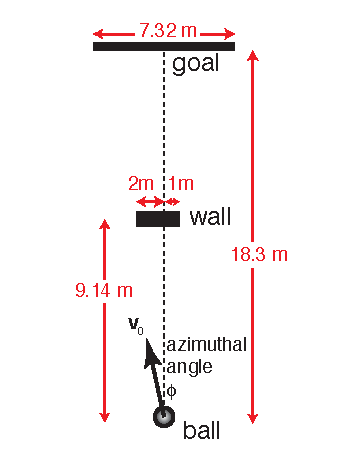
\includegraphics{figs/freekick-top}
    \caption{Top view. The initial velocity of the ball $\vec{v}_{0}$
      has an azimuthal (direction) angle $\phi$ that is positive when
      measured from the center line (dashed) in counterclockwise
      direction.}
    \label{fig:freekicktop}
  \end{subfigure}
  ~
  \begin{subfigure}[b]{0.4\linewidth}
    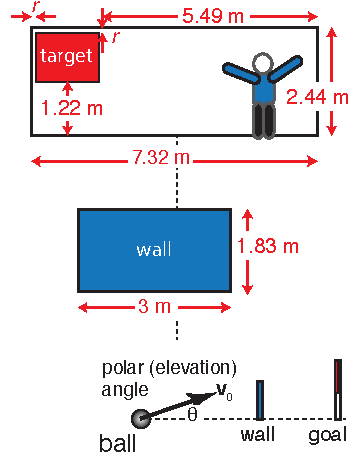
\includegraphics{figs/freekick-side}
    \caption{Side view. The initial velocity of the ball $\vec{v}_{0}$
      has a polar (launch) angle $\theta$ that is positive when
      measured above ground (dashed line).}
    \label{fig:freekickside}
  \end{subfigure}
  \caption{Sketch of the model for the free kick. The free kick is
    taken at the center at a distance of \SI{18.3}{m} from the
    goal. The wall made from defending players is positioned off
    center (dashed line) to guard the left half of the goal while the
    goal keeper defends the right half. The \emph{target} area for a
    scoring free kick (out of reach of the goalie and inside the goal)
    is in the upper left corner of the goal (as seen by the kicker);
    note that the target area is offset by the radius of the ball $r$
    from the top and left edges. The goal keeper is only shown for
    comparison.}
  \label{fig:freekick}
\end{figure}

The geometry for the \textbf{corner kick} is shown in
Fig.~\ref{fig:cornerkick}. We assume the kicker scores when she or he
can shoot the ball into the target area inside the goal near the far
post. In order to accomplish this, the ball must have some spin so
that it may curve back towards the goal.

\begin{figure}
  \centering
  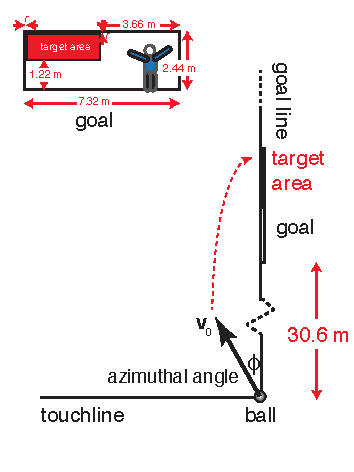
\includegraphics[width=0.5\linewidth]{figs/cornerkick-top.pdf}
  \caption{Sketch of the model for scoring from a corner kick. The
    ball has to be shot into the \emph{target area} (shown in the
    inset) near the far goal post (away from the corner). It is
    assumed that shots on goal but outside the target area can be
    easily caught by the goal keeper. For the shot to count as a goal,
    the ball may not cross the touchline or the goal line before
    entering the target area from the playing field side. The initial
    direction of the ball with velocity $\vec{v}_{0}$ is characterized
    by the azimuthal angle $\phi$ (in the plane of the field, here
    counted as positive into the field to the left) and the polar
    angle $\theta$ (launch angle measured from the ground up, not
    shown). Note that the target area is offset by the radius of the
    ball $r$ from the top and left edges. The goal keeper is only
    shown for comparison.}
  \label{fig:cornerkick}
\end{figure}





\subsection{Ball trajectories}
\label{sec:trajectories}

Your code should be able to generate realistic trajectories for balls
kicked in two set piece situations: the free kick (Section
\ref{sec:freekick}) and the corner kick (Section
\ref{sec:cornerkick}). You should plot a range of trajectories for
different initial conditions. The plots should show the elements on
the field (location of goal, target zone, and e.g., the wall of
defending players).

\subsubsection{Free kick}
\label{sec:freekick}

The geometry of the situation is described in
Fig.~\ref{fig:freekick}. A trajectory should start at the position of
the ball (\SI{18.3}{m} from the center of the goal). A trajectory
should end when the ball
\begin{enumerate}
\item leaves the field across the goal line
\item flies over the goal
\item crosses the goal line inside the goal (includes hitting the
  target area)
\item hits the wall
\end{enumerate}


\paragraph{Initial conditions}

Sensible ranges of parameters are \citep{Cook:2006aa}\footnote{For a
  related treatment of the problem see \citet{Bray:2003aa}.}
\begin{itemize}
\item initial velocity $\SI{24}{m.s^{-1}} \le v_{0} \le \SI{30}{m.s^{-1}}$
\item initial spin
  $\SI{0}{\revolutions\per\second} \le \omega_{0} \le
  \SI{12}{\revolutions\per\second}$ and for the orientation of the
  spin you may focus on full sideways spin, i.e., the spin axis
  $\boldsymbol{\omega}$ is perpendicular to the ground and parallel to
  the direction of gravity.
\item polar (launch) angle $\ang{10} \le \theta \le \ang{20}$
\item azimuthal (direction) angle $\ang{-2} \le \phi \le \ang{5}$
\end{itemize}

\subsubsection{Corner kick}
\label{sec:cornerkick}

The geometry of the situation is described in
Fig.~\ref{fig:cornerkick}. A trajectory should start at the position
of the ball on the corner of the field; assume that the ball sits on
the corner. A trajectory should end when the ball
\begin{enumerate}
\item leaves the field across the goal line or touchline
\item flies over the goal
\item crosses the goal line inside the goal (includes hitting the
  target area)
\end{enumerate}

\paragraph{Initial conditions}

Sensible starting ranges of parameters are shown below (based on
\citet{Cook:2006aa}) although you should feel to explore a wider range
of parameters if necessary.
\begin{itemize}
\item initial velocity $\SI{24}{m.s^{-1}} \le v_{0} \le
  \SI{30}{m.s^{-1}}$
\item initial spin
  $\SI{0}{\revolutions\per\second} \le \omega_{0} \le
  \SI{12}{\revolutions\per\second}$ and for the orientation of the
  spin you may focus on full sideways spin, i.e., the spin axis
  $\boldsymbol{\omega}$ is perpendicular to the ground and parallel to
  the direction of gravity.
\item polar (launch) angle $\ang{20} \le \theta \le \ang{30}$
\item azimuthal (direction) angle $\ang{-4} \le \phi \le \ang{4}$
\end{itemize}


\subsection{Goal-scoring trajectories}
\label{sec:scoring}

The aim of the project is to find parameters for the kicks that lead
to goals. In our model we consider a trajectory to be
\emph{goal-scoring} when it hits a \emph{target area}. This target
area is presumed to be a very difficult catch for the goal keeper. The
target areas are different for the two situations and are defined in
Figures \ref{fig:freekick} and \ref{fig:cornerkick}.

You can use any number of approaches to find goal-scoring
trajectories. Possible approaches are
\begin{description}
\item[exhaustive parameter scan] Run the simulation for combinations
  of parameters and store for each parameter combination if the
  trajectory was goal scoring; this is the approach taken by
  \citet{Cook:2006aa}.
\item[shooting algorithm] Combine the simulation algorithm with a root
  finding algorithm such as bisection to automatically find solutions
  to the problem; see Chapter 3.7 in \citet{Wang:2015aa}.
\item[manual experimentation] Manually rerun your simulation with
  different parameters, using intuition and previous trials to guide
  you. Record parameter sets that score a goal.
\end{description}
You are free to use whichever approach solves the problem, including
coming up with your own approach. However, you should not just ask
other students for the answer\dots (Make sure you read the notes on
the \emph{Acknowledgments} section in Section \ref{sec:report} below
if you heavily rely on the help of other people.)

At least one parameter set that leads to goal scoring trajectory
should be reported together with plots of the trajectory. The plots
must show clearly how the trajectory hits the target area.

\section{Report}
\label{sec:report}

Write a report in which you address the objectives in Section
\ref{sec:tasks} below in the context of the problem (Section
\ref{sec:problem}). The report should contain all results (figures,
tables, equations). It must contain a \emph{title}, \emph{author's
  name}, sections \emph{Background} (problem description, definitions,
any equations that you use), \emph{Results and Discussion}
(description and interpretation of results), and \emph{Summary} (short
summary of the main results).

The report \emph{must} contain a section \emph{Contributions} where
you summarize the contributions of each team member. For example, for
a team consisting of three members with initials A.B., C.D.E., and
F.G., the beginning of this section could be written along the lines
of
\begin{quotation}
  A.B.\ wrote the code to initialize the planet positions and
  velocities with help from C.D.E. C.D.E.\ wrote the integration
  routine, A.B., C.D.E., and F.G. together wrote the simulation
  function \texttt{simulate\_soccerball()}. F.G.\ with help from A.B.\
  wrote the orbit plotting code and produced figures 1 and 2. F.G.\
  also wrote the Background section \dots
\end{quotation}
(Note that all team members should have commits in the team
reporsitory.)

If you had any form of outside help you must describe it in an
\emph{Acknowledgments} section. 

If you use code or material from elsewhere you \emph{must cite the
  source} (add a \emph{References} section). 

Any bonus material can be shown in an optional \emph{Appendix}.

The report must be written in full sentences and read as a coherent
piece of work. Figures must have legends, labels, and captions. Type
set in an 11pt font with single line spacing (captions, labels, legend
may have smaller font sizes but must still be legible) and leave at
least 1~in margins. 

Overall, a length of about four pages is expected for a written
document produced with a word processor; the report should
not be less than three pages. The written portion (excluding figures)
should generally not exceed six pages.

\section{Code}
\label{sec:code}

For all numerical calculations use Python 3.x. You may use any of the
Python packages that are part of the Anaconda 3 distribution such as
\texttt{numpy} and \texttt{matplotlib}. 

\textbf{Include all the code that is needed to generate the results
  shown in your report.} This can consist of Python programs, modules,
a Jupyter notebook, or a mixture thereof. \textbf{Include a separate
  file \texttt{README.txt} that explains how to run your code} in
order to generate the results in your report. \textbf{Your code must
  run without errors} in order for you to be awarded full marks.


\section{Objectives}
\label{sec:tasks}
Address the following objectives in your report while taking all
requirements in Section \ref{sec:problem} into account:
\begin{enuma}
\item Briefly describe the behavior of the drag and lift coefficients
  of a soccer ball. Plot $C_{D}(v, S)$ (Eq.~\ref{eq:CDv}) in the range
  $0 < v < \SI{30}{m.s^{-1}}$ (1) for fixed $S=0$ and (2) for fixed
  $S=0.2$. Plot $C_{L}(S)$ (Eq.~\ref{eq:CL}) for $0 < S < 0.7$.
\item Simulate soccer ball trajectories of the
  \begin{enumi}
  \item \emph{free kick with wall} (\ref{sec:freekick}) and the
  \item \emph{corner kick} (\ref{sec:cornerkick})    
  \end{enumi}
 with your own Python program. 
\item For each case, show at least three typical trajectories using 2D
  plots (top and side views); as a bonus you can also show 3D
  plots. Describe the trajectories and list the parameters that were
  used to create them. ``Typical'' means that they should show a broad
  range of outcomes such as ``hits the goal'', ``hits the wall'',
  ``flies besides or over the goal'', \dots.
\item For each of the two cases, find at least one set of parameters
  that results in a \emph{goal-scoring trajectory} (see Section
  \ref{sec:scoring}). For each goal-scoring trajectory
  \begin{enumi}    
  \item list the parameters
  \item show plots of the trajectory
  \item include a plot of a trajectory with the same parameters as the
    scoring trajectory \emph{except} that spin is set to zero
    ($\omega_{0} = 0$) to demonstrate the influence of spin
  \end{enumi}
\end{enuma}

\section{History}
\label{sec:history}

Changes and updates to this document.
\begin{description}
\item[2018-03-26] initial version
\end{description}
  
\bibliographystyle{physbiol-natbib}      % basic style, author-year citations
\bibliography{phy494}   % name your BibTeX data base

\end{document}

%%% Local Variables: 
%%% mode: latex
%%% TeX-master: t
%%% End: 
